%% DH-412 Presentation — Part 4: Working with the Data
%% Weilun Xu's slides only
\documentclass[aspectratio=169]{beamer}

\usetheme{Madrid}
\usecolortheme{crane}
\setbeamertemplate{navigation symbols}{}
\setbeamertemplate{footline}[frame number]

\usepackage{booktabs}
\usepackage{graphicx}

\title{How We Envisage Working with the Data}
\subtitle{\textit{Framing} and \textit{Reframing} Iran in the \textit{New York Times}}
\author{Weilun Xu}
\institute{DH-412 --- EPFL}
\date{Spring 2026}

\begin{document}

%% ─────────────────────────────────
%% SLIDE 1: WHAT THE DATA ALREADY SHOWS
%% ─────────────────────────────────
\begin{frame}{What the Data Already Reveals}
  \begin{center}
    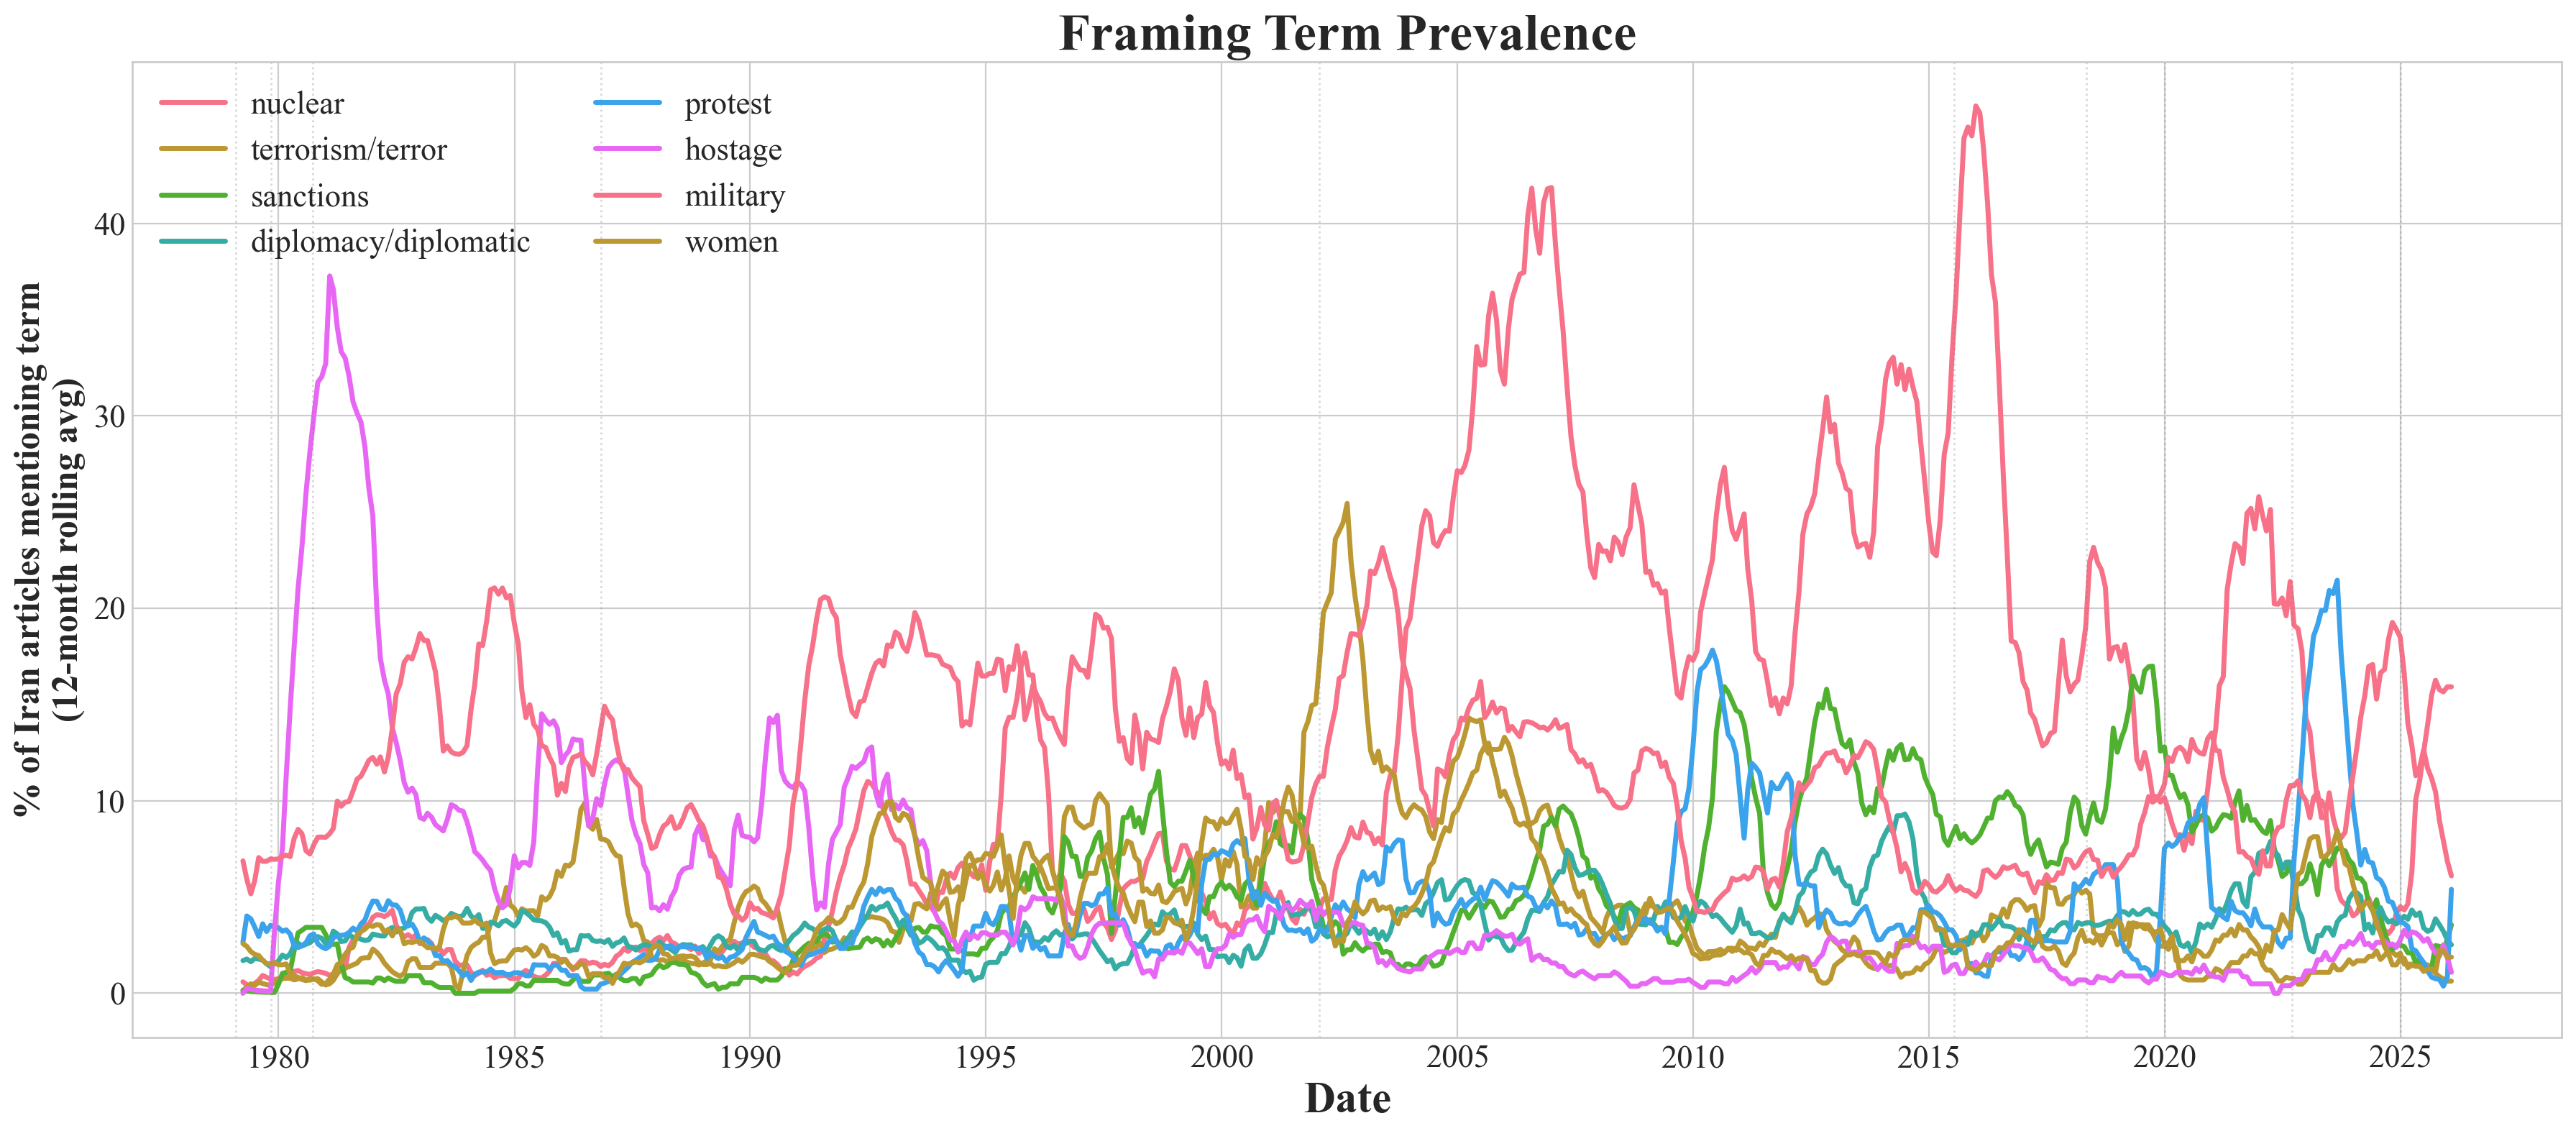
\includegraphics[width=\linewidth]{../figures/eda_pres/03_keyword_trends.png}
  \end{center}
  \vspace{-0.5em}
  \small Keyword prevalence (12-month rolling avg) shows \textbf{frame succession}: dominant frames shift from ``hostage'' (37\%) $\to$ ``nuclear'' (45\%) $\to$ ``Israel'' (49\%), while \textbf{``diplomacy'' never exceeds 7\%}.
\end{frame}

%% ─────────────────────────────────
%% SLIDE 2: METHODS OVERVIEW
%% ─────────────────────────────────
\begin{frame}{Envisaged Methods}
  \begin{columns}[T]
    \begin{column}{0.55\textwidth}
      \textbf{For RQ1 (Frame Discontinuities):}
      \begin{itemize}
        \item \textbf{BERTopic} for dynamic topic modeling --- track how thematic clusters evolve across decades
        \item \textbf{Sentiment analysis} (transformer-based) for headline-level affect
        \item \textbf{Structural break detection} to identify statistically significant framing shifts at geopolitical turning points
      \end{itemize}
      \vspace{0.5em}
      \textbf{For RQ2 (Re-narration):}
      \begin{itemize}
        \item Keyword \textbf{co-occurrence analysis} across temporal layers --- how vocabulary applied to past events changes over time
      \end{itemize}
    \end{column}
    \begin{column}{0.45\textwidth}
      \textbf{For RQ3 (Genre \& Theme):}
      \begin{itemize}
        \item Compare framing across \textbf{news vs.\ opinion} using section/desk metadata
        \item Cross-tabulate topics with thematic contexts (political, cultural, protest, nuclear)
      \end{itemize}
      \vspace{0.5em}
      \textbf{Visual Analysis:}
      \begin{itemize}
        \item Annotate stratified \textbf{image sample}
        \item Cross-tabulate visual content categories with textual framing scores
        \item Examine visual--textual tension
      \end{itemize}
    \end{column}
  \end{columns}
\end{frame}

%% ─────────────────────────────────
%% SLIDE 3: RE-NARRATION EVIDENCE + TEST CASES
%% ─────────────────────────────────
\begin{frame}{Re-narration Signals \& Key Test Cases}
  \begin{columns}[T]
    \begin{column}{0.5\textwidth}
      \begin{center}
        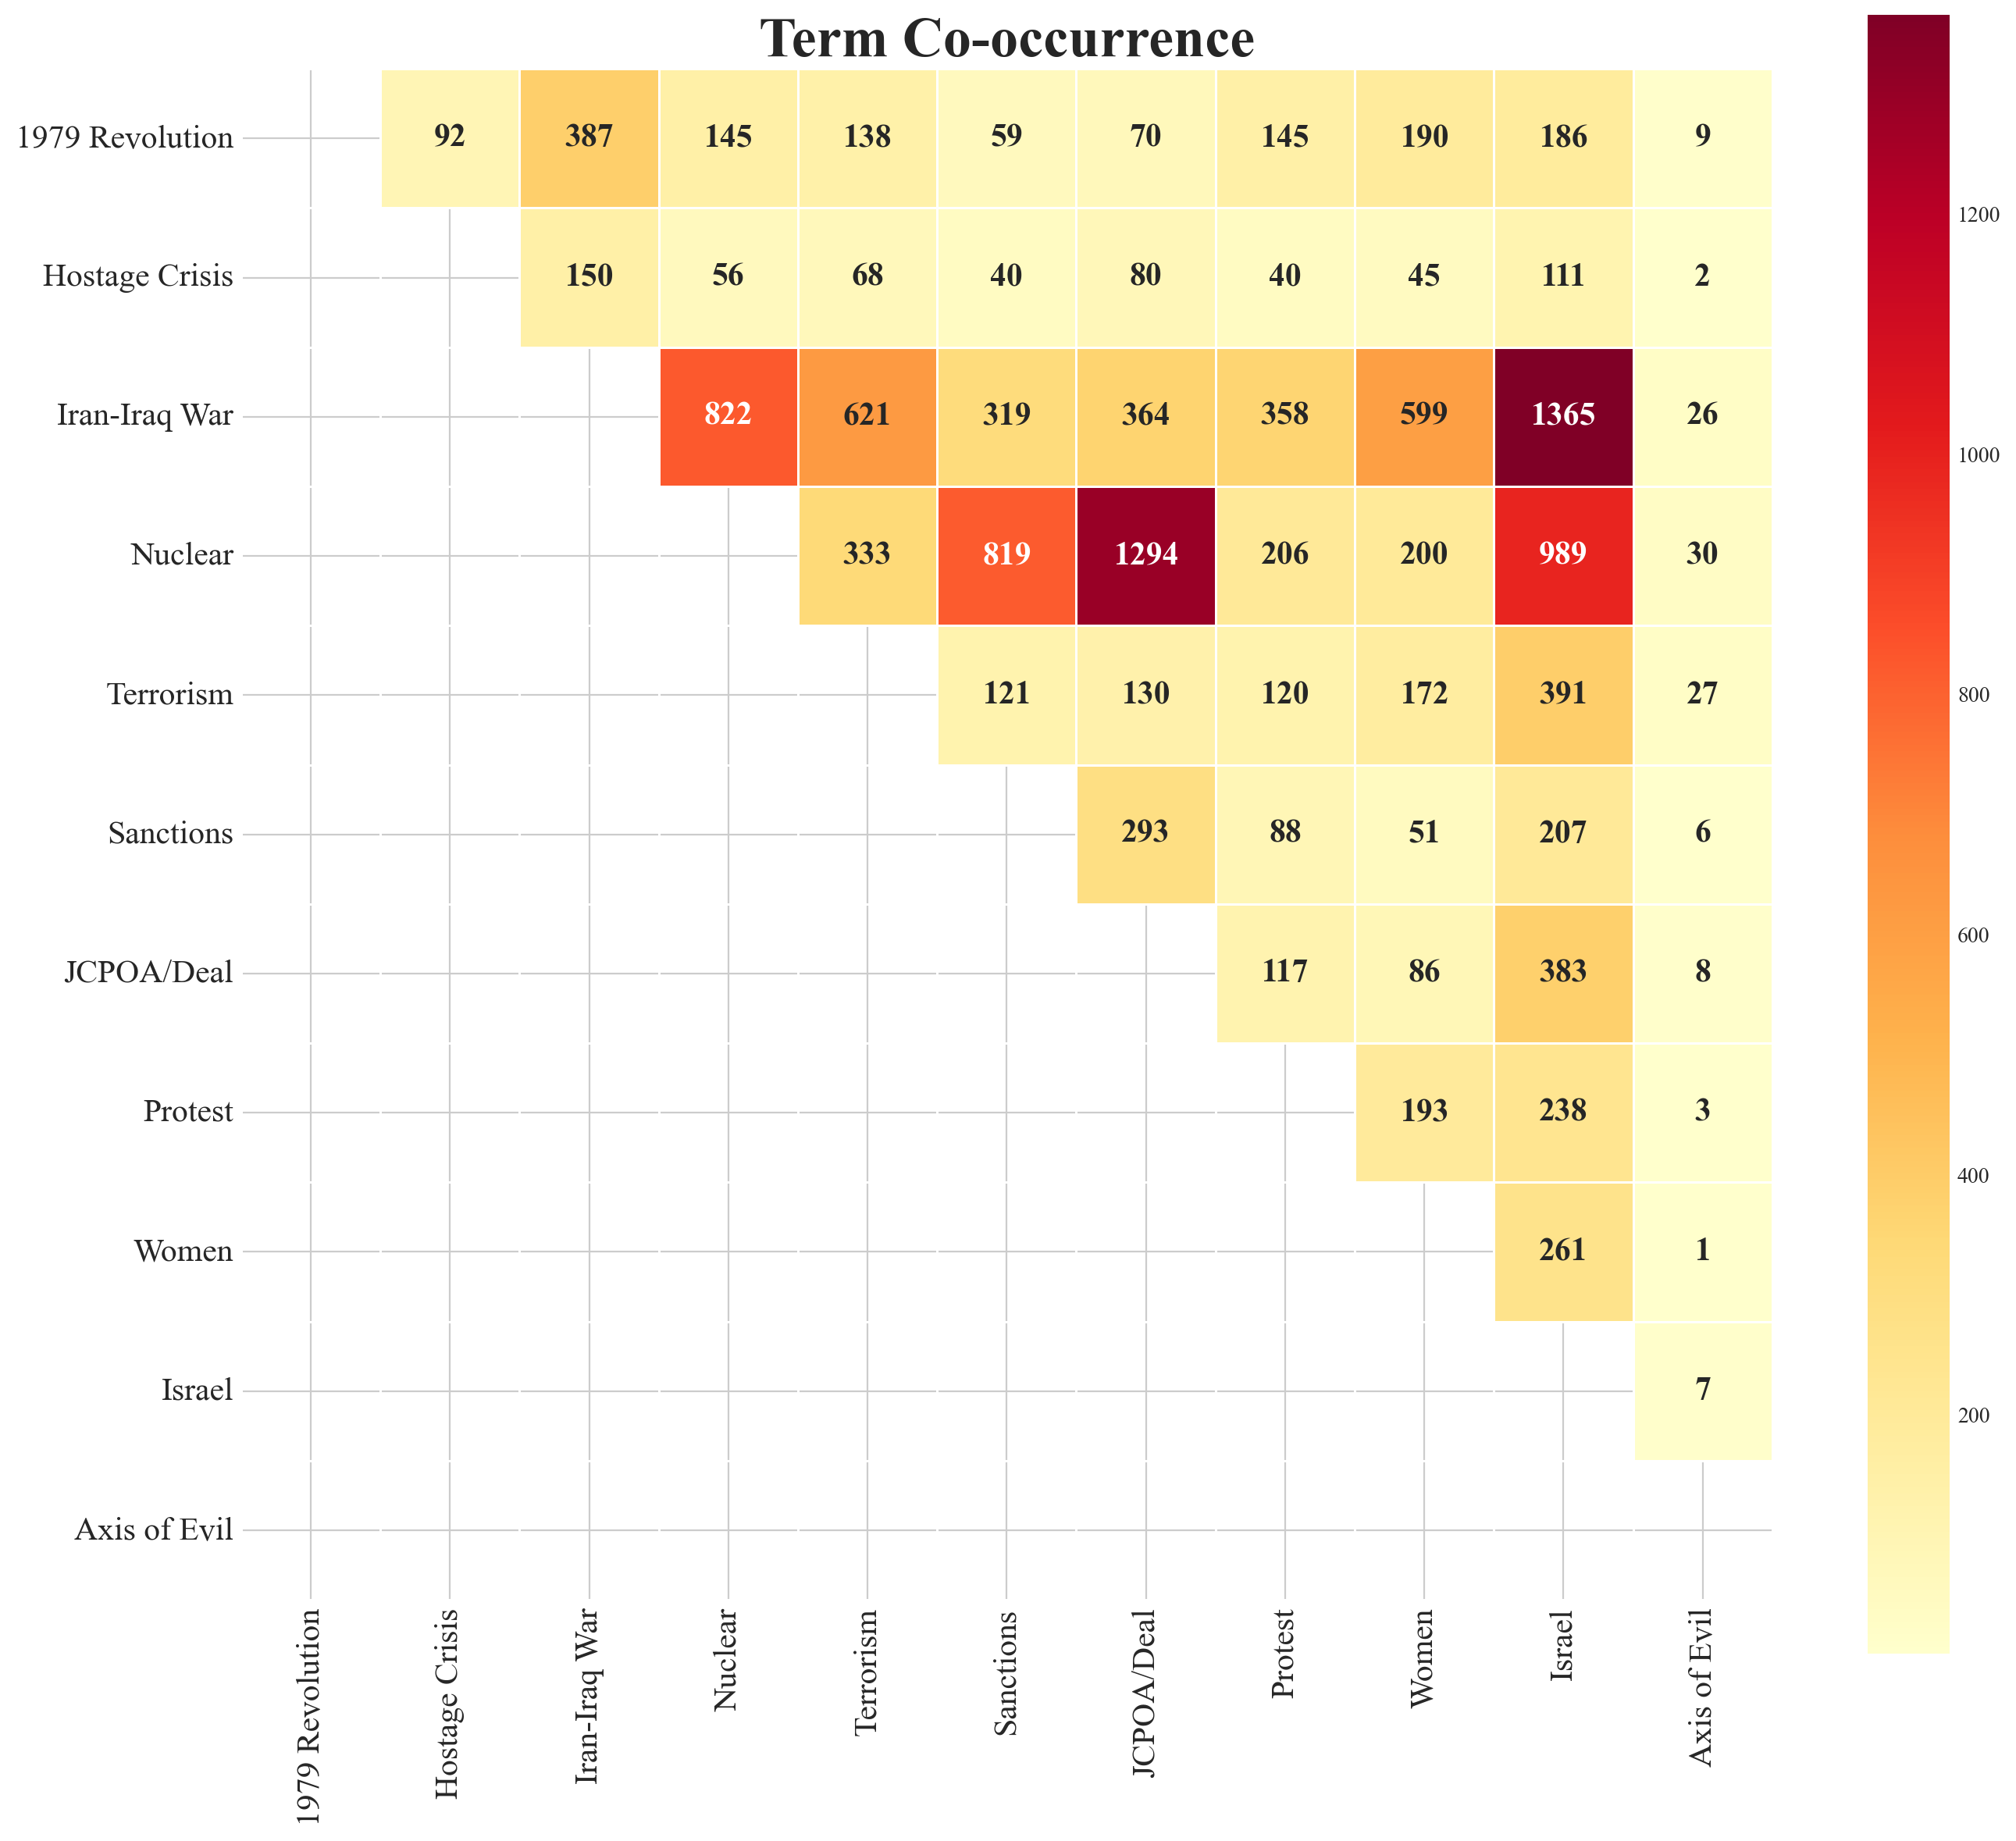
\includegraphics[width=\linewidth]{../figures/eda_pres/08_cooccurrence.png}
      \end{center}
      \vspace{-0.5em}
      \small Co-occurrence heatmap: e.g.\ 387 articles link ``revolution'' with ``hostage,'' 145 with ``nuclear'' --- evidence of retroactive re-framing.
    \end{column}
    \begin{column}{0.5\textwidth}
      \textbf{Critical test cases:}
      \vspace{0.5em}
      \begin{itemize}
        \item \textbf{2022 WLF protests:}\\Does framing shift toward internal politics and civil rights?
        \vspace{0.5em}
        \item \textbf{2024--25 Israel--Iran conflict:}\\Does ``Israel'' become the new dominant frame, extending the succession pattern?
        \vspace{0.5em}
        \item \textbf{Or do new narrative structures emerge?}\\Breaking the hostage $\to$ nuclear $\to$ ? pattern
      \end{itemize}
    \end{column}
  \end{columns}
\end{frame}

\end{document}
